\documentclass[preprint,12pt,aps,pra,showkeys,amsmath,amssymb,superscriptaddress,floatfix]{revtex4-2}
\usepackage[T1]{fontenc}
\usepackage[utf8]{inputenc}
\usepackage{amsmath,amssymb,amsthm,mathtools,mathrsfs}
\usepackage{microtype,booktabs,enumitem}
\usepackage{xcolor,tikz,etoolbox}
\usepackage[skins,breakable]{tcolorbox}
\usepackage{needspace}
% Keep diagram geometry independent of REVTeX preprint body spacing.
\AtBeginEnvironment{tikzpicture}{\linespread{1}\selectfont}
\usetikzlibrary{arrows.meta,positioning,calc,fit,decorations.pathreplacing}
\usepackage{graphicx}
\usepackage{hyperref}

\definecolor{MMBlue}{RGB}{0,82,155}
\definecolor{MMOrange}{RGB}{200,80,0}
\tikzset{
 mmnode/.style={draw=MMBlue,rounded corners=2pt,fill=MMBlue!4,align=left,execute at begin node={\raggedright},text width=5cm,font=\fontsize{10}{12}\selectfont,inner sep=6pt},
 mmimport/.style={mmnode,draw=black!65,fill=black!4},
 mmcandidate/.style={mmnode,draw=MMOrange,dashed,fill=MMOrange!5},
 mmrejected/.style={mmnode,draw=black,densely dotted,fill=black!8},
 mmproof/.style={->,thick,MMBlue},
 mmflow/.style={->,semithick,black!70},
 mmrepair/.style={->,dashed,thick,MMOrange},
 mmcandidatearrow/.style={->,dashed,semithick,MMOrange},
 mmnote/.style={font=\scriptsize,fill=white,inner sep=2pt,align=center}}

\usepackage[section]{placeins}
\setlength{\emergencystretch}{3em}
\setlist{itemsep=3pt,topsep=4pt}
\newtheorem{theorem}{Theorem}[section]
\newtheorem{proposition}[theorem]{Proposition}
\newtheorem{lemma}[theorem]{Lemma}
\newtheorem{corollary}[theorem]{Corollary}
\theoremstyle{definition}
\newtheorem{definition}[theorem]{Definition}
\newtheorem{example}[theorem]{Example}
\theoremstyle{remark}
\newtheorem{remark}[theorem]{Remark}
% Avoid isolated statement headings and single-line paragraph fragments.
\BeforeBeginEnvironment{theorem}{\Needspace{6\baselineskip}}
\BeforeBeginEnvironment{definition}{\Needspace{5\baselineskip}}
\BeforeBeginEnvironment{proposition}{\Needspace{5\baselineskip}}
\BeforeBeginEnvironment{lemma}{\Needspace{5\baselineskip}}
\BeforeBeginEnvironment{corollary}{\Needspace{5\baselineskip}}
\clubpenalty=5000
\widowpenalty=5000
\newcommand{\R}{\mathbb R}\newcommand{\Z}{\mathbb Z}\newcommand{\N}{\mathbb N}
\newcommand{\Pa}{\operatorname{Pa}}\newcommand{\Desc}{\operatorname{Desc}}
\newcommand{\cl}{\operatorname{cl}}\newcommand{\cost}{\operatorname{cost}}
\newcommand{\status}{\operatorname{status}}
% Faculty cards: a visual rail groups the five faculties within one agent.
% The rail has no arrowhead and does not represent a proof dependency.
\newcommand{\mmfacultybadge}[1]{%
 \node[circle,draw=MMBlue,line width=1pt,fill=white,
 minimum size=7mm,inner sep=0pt,font=\sffamily\small\bfseries,text=MMBlue]
 at ([xshift=15pt,yshift=-15pt]frame.north west) {#1};}
\newcommand{\mmfacultyrail}{%
 \draw[MMBlue!80,line width=1pt]
 ([xshift=15pt,yshift=2pt]frame.north west)--
 ([xshift=15pt,yshift=-2pt]frame.south west);}
\newtcolorbox{mmfacultybox}[2]{enhanced,breakable,
 colback=MMBlue!4,colframe=MMBlue!4,boxrule=0pt,arc=3pt,
 left=39pt,right=9pt,top=4pt,bottom=4pt,
 before skip=2pt,after skip=2pt,
 fontupper=\small\linespread{1.1}\selectfont,
 overlay unbroken={\mmfacultyrail\mmfacultybadge{#1}},
 overlay first={\mmfacultyrail\mmfacultybadge{#1}},
 overlay middle={\mmfacultyrail},overlay last={\mmfacultyrail}}
\newcommand{\mmfaculty}[3]{%
 \begin{mmfacultybox}{#1}{#2}
 {\sffamily\bfseries\color{MMBlue}#2}\par\smallskip #3
 \end{mmfacultybox}}
\newcommand{\agent}[9]{%
 \Needspace{8\baselineskip}
 \subsubsection{#1}
 \noindent\textbf{Object.} #2\par
 \noindent\textbf{Role.} #3\par\smallskip
 \mmfaculty{E}{Ego}{#4}
 \mmfaculty{M}{Memory}{#5}
 \mmfaculty{I}{Intellect}{#6}
 \mmfaculty{S}{Sense}{#7}
 \mmfaculty{A}{Action}{#8}
 \smallskip\noindent #9\par}

\usepackage{longtable,array,calc}
\providecommand{\tightlist}{\setlength{\itemsep}{2pt}\setlength{\parskip}{0pt}}
\makeatletter
\def\frontmatter@abstract@produce{\par\addvspace{\frontmatter@preabstractspace}%
\begingroup\prep@absbox\unvbox\absbox\post@absbox\endgroup
\addvspace{\frontmatter@postabstractspace}}
\makeatother
\newcommand{\field}[2]{\par\smallskip\noindent\textbf{#1.} #2\par}
\setlength{\emergencystretch}{5em}
\AtBeginEnvironment{verbatim}{\small\linespread{1.0}\selectfont}


\hypersetup{colorlinks=true,linkcolor=MMBlue,urlcolor=MMBlue,pdfauthor={Dibakar Sigdel}}

\begin{document}

\title{First-Order Compactness via Ultraproducts\\[4pt]\large An End-to-End Meta-Math Walkthrough}

\author{Dibakar Sigdel}

\affiliation{Mindverse Computing LLC, Lynnwood, WA 98087, USA}

\date{October 2026}

\begin{abstract}

Each finite fragment gets its own model. An ultrafilter regards all
fragments containing any chosen sentence as large; the quotient product
then makes every sentence in the theory true at once. The report
presents the target theorem, declared imports, a dependency graph,
five-faculty node contracts, a continuous proof, a worked example, and a
hypothesis-repair audit. It is an authored mathematical exposition, not
a deployed-agent transcript or a formal proof-assistant certificate.

\end{abstract}\maketitle\linespread{1.12}\selectfont

\noindent\textbf{LF-03 / Mathematical Logic and Set Theory / Report v1}

\section{Target and import contract}

\begin{theorem}

Let \(T\) be a set of sentences in a first-order language \(L\) with
finite-arity relation and function symbols and nonempty structures. If
every finite subset of \(T\) has a model, prove \(T\) has a model. Work
in classical ZFC set theory, including choice. The proof constructs an
ultraproduct and proves the required truth-transfer lemma rather than
importing first-order completeness.

\end{theorem}

\subsection{Foundations and permitted imports}

Use Zorn's lemma, choice of structures and witnesses from set-indexed
nonempty families, finite-intersection filters, and the recursive
semantics of first-order formulas. A proper filter on an index set
contains the whole set, not the empty set, and is closed under finite
intersections and supersets. An ultrafilter is a maximal proper filter.
Function symbols may include zero-arity constants. General formulas can
be expressed using atomic formulas, negation, conjunction, and
existential quantification.

\clearpage\section{Node interaction workflow}

\begin{center}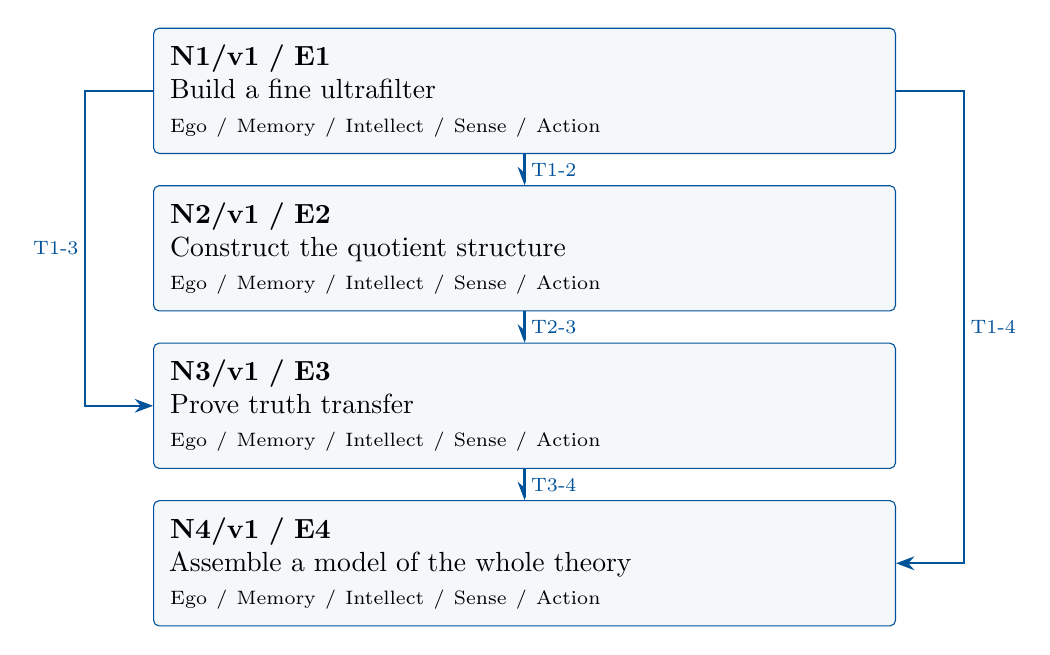
\begin{tikzpicture}[>=Stealth,x=1cm,y=1cm]

\node[mmnode,text width=9cm,minimum height=1.25cm] (N1) at (0,0.0) {\textbf{N1/v1 / E1}\\Build a fine ultrafilter\\{\scriptsize Ego / Memory / Intellect / Sense / Action}};

\node[mmnode,text width=9cm,minimum height=1.25cm] (N2) at (0,-2.0) {\textbf{N2/v1 / E2}\\Construct the quotient structure\\{\scriptsize Ego / Memory / Intellect / Sense / Action}};

\node[mmnode,text width=9cm,minimum height=1.25cm] (N3) at (0,-4.0) {\textbf{N3/v1 / E3}\\Prove truth transfer\\{\scriptsize Ego / Memory / Intellect / Sense / Action}};

\node[mmnode,text width=9cm,minimum height=1.25cm] (N4) at (0,-6.0) {\textbf{N4/v1 / E4}\\Assemble a model of the whole theory\\{\scriptsize Ego / Memory / Intellect / Sense / Action}};

\draw[mmproof] (N1.south) -- node[mmnote,right] {T1-2} (N2.north);

\draw[mmproof] (N1.west) -- (-5.58,0) -- node[mmnote,left] {T1-3} (-5.58,-4) -- (N3.west);

\draw[mmproof] (N2.south) -- node[mmnote,right] {T2-3} (N3.north);

\draw[mmproof] (N1.east) -- (5.58,0) -- node[mmnote,right] {T1-4} (5.58,-6) -- (N4.east);

\draw[mmproof] (N3.south) -- node[mmnote,right] {T3-4} (N4.north);

\end{tikzpicture}\end{center}

Each box is one mathematical agent containing all five faculties. Blue
arrows carry the versioned exports listed below. The layout gives a
reading order; only drawn arrows assert dependencies. Diagnostic repair
is separate from the proof DAG.

\clearpage\subsection{Versioned evidence-transfer ledger}

\begingroup\small\linespread{1.05}\selectfont

\Needspace{5\baselineskip}\field{T1-2: N1/E1/v1 to N2}{There is an ultrafilter \(\mathcal U\) on \(I\) containing every
\(C_\varphi\), and exactly one of \(A,I\setminus A\) belongs to
\(\mathcal U\) for each \(A\subset I\).}

\field{Receiving activity}{N2.1}

\field{Compatibility}{E1/v1; choose a nonempty model \(M_s\models s\) for each \(s\in I\).
Check: Finite intersections, not countable intersections, suffice for
each finite-arity symbol; representatives must not affect truth or
function values.}

\Needspace{5\baselineskip}\field{T1-3: N1/E1/v1 to N3}{There is an ultrafilter \(\mathcal U\) on \(I\) containing every
\(C_\varphi\), and exactly one of \(A,I\setminus A\) belongs to
\(\mathcal U\) for each \(A\subset I\).}

\field{Receiving activity}{N3.1}

\field{Compatibility}{E1/v1 and E2/v1, a first-order formula \(\theta\), and product
representatives for its finitely many parameters. Check: Existential
witnesses may vary with the index. Requiring one common element of all
models would be an invalid strengthening.}

\Needspace{5\baselineskip}\field{T2-3: N2/E2/v1 to N3}{The product modulo \(a\sim b\iff\{s:a_s=b_s\}\in\mathcal U\) is a
well-defined nonempty \(L\)-structure \(M\).}

\field{Receiving activity}{N3.1}

\field{Compatibility}{E1/v1 and E2/v1, a first-order formula \(\theta\), and product
representatives for its finitely many parameters. Check: Existential
witnesses may vary with the index. Requiring one common element of all
models would be an invalid strengthening.}

\Needspace{5\baselineskip}\field{T1-4: N1/E1/v1 to N4}{There is an ultrafilter \(\mathcal U\) on \(I\) containing every
\(C_\varphi\), and exactly one of \(A,I\setminus A\) belongs to
\(\mathcal U\) for each \(A\subset I\).}

\field{Receiving activity}{N4.1}

\field{Compatibility}{E1/v1 cones and E3/v1 truth transfer for sentences. Check: The final
assertion quantifies over every sentence separately; no infinite
intersection in the ultrafilter is required.}

\Needspace{5\baselineskip}\field{T3-4: N3/E3/v1 to N4}{\(M\models\theta([a^1],\ldots,[a^r])\) iff
\(\{s:M_s\models\theta(a_s^1,\ldots,a_s^r)\}\in\mathcal U\).}

\field{Receiving activity}{N4.2}

\field{Compatibility}{E1/v1 cones and E3/v1 truth transfer for sentences. Check: The final
assertion quantifies over every sentence separately; no infinite
intersection in the ultrafilter is required.}

\endgroup

\clearpage\section{Agent roles and five-faculty activities}\begingroup\small\linespread{1.05}\selectfont\setlist{itemsep=1pt,topsep=2pt}

\begingroup\footnotesize\linespread{1.05}\selectfont\let\small\footnotesize

\subsection{N1/v1: Build a fine ultrafilter}

\field{Object and role}{Extend the filter generated by the cones to an ultrafilter and derive
its complement decision property. \textbf{Local obligation:} There is an
ultrafilter \(\mathcal U\) on \(I\) containing every \(C_\varphi\), and
exactly one of \(A,I\setminus A\) belongs to \(\mathcal U\) for each
\(A\subset I\).}

\field{Inputs}{\(I=\{s\subset T:s\text{ finite}\}\) and
\(C_\varphi=\{s\in I:\varphi\in s\}\) for \(\varphi\in T\).}

\mmfaculty{E}{Ego}{Publish E1/v1 only after establishing this obligation: There is an
ultrafilter \(\mathcal U\) on \(I\) containing every \(C_\varphi\), and
exactly one of \(A,I\setminus A\) belongs to \(\mathcal U\) for each
\(A\subset I\).}

\mmfaculty{M}{Memory}{\(I=\{s\subset T:s\text{ finite}\}\) and
\(C_\varphi=\{s\in I:\varphi\in s\}\) for \(\varphi\in T\). Retain the
stated assumptions and import versions.}

\mmfaculty{I}{Intellect}{Extend the filter generated by the cones to an ultrafilter and derive
its complement decision property.}

\mmfaculty{S}{Sense}{Every finite intersection of cones contains their finite list of
sentences as an index, so it is nonempty.}

\mmfaculty{A}{Action}{Carry out activities N1.1--N1.2 below, retaining each calculation and
construction as evidence.}

\smallskip\noindent\textbf{Numbered mathematical activities}

\begin{enumerate}[label=N1.\arabic*,leftmargin=3.4em]

\item Finite intersections of the cones are nonempty: the finite union of the
required sentences is itself an index. They therefore generate a proper
filter (if \(T\) is empty use the filter containing \(I\)). The union of
a chain of proper filters is again a proper filter, because any finitely
many of its members occur together in one member of the chain. Zorn
supplies a maximal proper filter \(\mathcal U\).

\item If \(A\notin\mathcal U\), adjoining it cannot generate a proper larger
filter. Thus some \(F\in\mathcal U\) has \(F\cap A=\varnothing\);
otherwise its intersections with old filter members would give a proper
extension. Therefore \(I\setminus A\in\mathcal U\). Both complementary
sets cannot belong, since their intersection is empty. This is the
required decision property.

\end{enumerate}

\field{Export E1/v1}{There is an ultrafilter \(\mathcal U\) on \(I\) containing every
\(C_\varphi\), and exactly one of \(A,I\setminus A\) belongs to
\(\mathcal U\) for each \(A\subset I\).}

\field{Acceptance gate}{Every finite intersection of cones contains their finite list of
sentences as an index, so it is nonempty.}

\field{Targeted repair}{If maximality is used without a chain upper bound, supply the
union-of-chain argument and check that the empty set never enters.
Withhold this export and recheck its descendants after a versioned
correction.}

\endgroup

\clearpage

\begingroup\footnotesize\linespread{1.05}\selectfont\let\small\footnotesize

\subsection{N2/v1: Construct the quotient structure}

\field{Object and role}{Quotient the product by agreement on an ultrafilter-large set and define
symbols coordinatewise. \textbf{Local obligation:} The product modulo
\(a\sim b\iff\{s:a_s=b_s\}\in\mathcal U\) is a well-defined nonempty
\(L\)-structure \(M\).}

\field{Inputs}{E1/v1; choose a nonempty model \(M_s\models s\) for each \(s\in I\).
Incoming proof exports: E1/v1 at N2.1.}

\mmfaculty{E}{Ego}{Publish E2/v1 only after establishing this obligation: The product
modulo \(a\sim b\iff\{s:a_s=b_s\}\in\mathcal U\) is a well-defined
nonempty \(L\)-structure \(M\).}

\mmfaculty{M}{Memory}{E1/v1; choose a nonempty model \(M_s\models s\) for each \(s\in I\).
Incoming proof exports: E1/v1 at N2.1. Retain the stated assumptions and
import versions.}

\mmfaculty{I}{Intellect}{Quotient the product by agreement on an ultrafilter-large set and define
symbols coordinatewise.}

\mmfaculty{S}{Sense}{Finite intersections, not countable intersections, suffice for each
finite-arity symbol; representatives must not affect truth or function
values.}

\mmfaculty{A}{Action}{Carry out activities N2.1--N2.2 below, retaining each calculation and
construction as evidence.}

\smallskip\noindent\textbf{Numbered mathematical activities}

\begin{enumerate}[label=N2.\arabic*,leftmargin=3.4em]

\item Choice gives the family of models and an element in each domain, so
their product is nonempty. Agreement is reflexive and symmetric;
transitivity follows because the intersection of two large agreement
sets is large and is contained in the third agreement set. Thus \(\sim\)
is an equivalence relation.

\item Interpret a function on classes by applying it in each \(M_s\), and
interpret a relation \(R([a^1],\ldots,[a^r])\) as true when
\(\{s:M_s\models R(a_s^1,\ldots,a_s^r)\}\in\mathcal U\). If
representatives change, they agree on the finite intersection of their
large agreement sets. Function outputs and relation truth agree there,
so their quotient value or largeness is unchanged. Equality is the
equivalence relation itself; constants are their coordinatewise classes.
This defines \(M\).

\end{enumerate}

\field{Export E2/v1}{The product modulo \(a\sim b\iff\{s:a_s=b_s\}\in\mathcal U\) is a
well-defined nonempty \(L\)-structure \(M\).}

\field{Acceptance gate}{Finite intersections, not countable intersections, suffice for each
finite-arity symbol; representatives must not affect truth or function
values.}

\field{Targeted repair}{If infinitely many representative agreements are intersected for one
formula, use only its finite tuple of free variables and the finite
arities actually present. Withhold this export and recheck its
descendants after a versioned correction.}

\endgroup

\clearpage

\begingroup\linespread{1}\fontsize{9.5}{11}\selectfont\renewcommand{\small}{\fontsize{9.5}{11}\selectfont}

\subsection{N3/v1: Prove truth transfer}

\field{Object and role}{Induct on terms and formula construction; use chosen witnesses for the
existential direction. \textbf{Local obligation:}
\(M\models\theta([a^1],\ldots,[a^r])\) iff
\(\{s:M_s\models\theta(a_s^1,\ldots,a_s^r)\}\in\mathcal U\).}

\field{Inputs}{E1/v1 and E2/v1, a first-order formula \(\theta\), and product
representatives for its finitely many parameters. Incoming proof
exports: E1/v1 at N3.1, E2/v1 at N3.1.}

\mmfaculty{E}{Ego}{Publish E3/v1 only after establishing this obligation:
\(M\models\theta([a^1],\ldots,[a^r])\) iff
\(\{s:M_s\models\theta(a_s^1,\ldots,a_s^r)\}\in\mathcal U\).}

\mmfaculty{M}{Memory}{E1/v1 and E2/v1, a first-order formula \(\theta\), and product
representatives for its finitely many parameters. Incoming proof
exports: E1/v1 at N3.1, E2/v1 at N3.1. Retain the stated assumptions and
import versions.}

\mmfaculty{I}{Intellect}{Induct on terms and formula construction; use chosen witnesses for the
existential direction.}

\mmfaculty{S}{Sense}{Existential witnesses may vary with the index. Requiring one common
element of all models would be an invalid strengthening.}

\mmfaculty{A}{Action}{Carry out activities N3.1--N3.3 below, retaining each calculation and
construction as evidence.}

\smallskip\noindent\textbf{Numbered mathematical activities}

\begin{enumerate}[label=N3.\arabic*,leftmargin=3.4em]

\item Induction on terms shows evaluation is coordinatewise up to \(\sim\):
variables and constants have this property by definition, and applying a
function preserves it. Atomic equality and relations therefore satisfy
the asserted transfer by N2. Negation corresponds to complement, handled
by the ultrafilter decision property. Conjunction corresponds to
intersection; a finite intersection is large exactly when both factors
are large, by filter closure and upward closure.

\item For \(\exists z\,\psi(z,\bar a)\), first suppose \(M\) has a witnessing
class \([b]\). By the induction hypothesis,
\(\{s:M_s\models\psi(b_s,\bar a_s)\}\) is large. It is contained in the
set of indices satisfying the existential formula, so that set is large.

\item Conversely, if the existential satisfaction set is large, choose a
witness \(b_s\) in each of its models, and choose an arbitrary domain
element at the remaining indices. Choice and nonempty domains permit
this product element. The set where \(\psi(b_s,\bar a_s)\) holds
contains the large existential set. The induction hypothesis then makes
\([b]\) a witness in \(M\). These cases complete the structural
induction and prove truth transfer.

\end{enumerate}

\field{Export E3/v1}{\(M\models\theta([a^1],\ldots,[a^r])\) iff
\(\{s:M_s\models\theta(a_s^1,\ldots,a_s^r)\}\in\mathcal U\).}

\field{Acceptance gate}{Existential witnesses may vary with the index. Requiring one common
element of all models would be an invalid strengthening.}

\field{Targeted repair}{If the existential case is dismissed as automatic, construct the
coordinatewise witnesses and explicitly use the induction hypothesis for
the matrix formula. Withhold this export and recheck its descendants
after a versioned correction.}

\endgroup

\clearpage

\subsection{N4/v1: Assemble a model of the whole theory}

\field{Object and role}{Use each sentence's cone as a subset of its satisfaction set.
\textbf{Local obligation:} \(M\models T\), proving compactness.}

\field{Inputs}{E1/v1 cones and E3/v1 truth transfer for sentences. Incoming proof
exports: E1/v1 at N4.1, E3/v1 at N4.2.}

\mmfaculty{E}{Ego}{Publish E4/v1 only after establishing this obligation: \(M\models T\),
proving compactness.}

\mmfaculty{M}{Memory}{E1/v1 cones and E3/v1 truth transfer for sentences. Incoming proof
exports: E1/v1 at N4.1, E3/v1 at N4.2. Retain the stated assumptions and
import versions.}

\mmfaculty{I}{Intellect}{Use each sentence's cone as a subset of its satisfaction set.}

\mmfaculty{S}{Sense}{The final assertion quantifies over every sentence separately; no
infinite intersection in the ultrafilter is required.}

\mmfaculty{A}{Action}{Carry out activities N4.1--N4.2 below, retaining each calculation and
construction as evidence.}

\smallskip\noindent\textbf{Numbered mathematical activities}

\begin{enumerate}[label=N4.\arabic*,leftmargin=3.4em]

\item Fix \(\varphi\in T\). Whenever \(s\in C_\varphi\), the chosen \(M_s\) is
a model of \(s\), so it satisfies \(\varphi\). Therefore
\(C_\varphi\subset\{s:M_s\models\varphi\}\). The left side is large by
N1, hence so is the right side.

\item By N3, \(M\models\varphi\). Since this holds for every \(\varphi\in T\),
\(M\models T\). No common index need satisfy all of \(T\); the quotient
construction is what supplies the new model.

\end{enumerate}

\field{Export E4/v1}{\(M\models T\), proving compactness.}

\field{Acceptance gate}{The final assertion quantifies over every sentence separately; no
infinite intersection in the ultrafilter is required.}

\field{Targeted repair}{If all cones are intersected and assumed large, replace that step by
one-sentence-at-a-time truth transfer; filters are only finitely
intersection-closed. Withhold this export and recheck its descendants
after a versioned correction.}

\endgroup\clearpage\section{Continuous mathematical proof}\label{sec:proof}

\subsection{N1 --- Build a fine
ultrafilter}\label{n1-build-a-fine-ultrafilter}

\begin{enumerate}
\def\labelenumi{\arabic{enumi}.}
\item
  \textbf{N1.1.} Finite intersections of the cones are nonempty: the
  finite union of the required sentences is itself an index. They
  therefore generate a proper filter (if \(T\) is empty use the filter
  containing \(I\)). The union of a chain of proper filters is again a
  proper filter, because any finitely many of its members occur together
  in one member of the chain. Zorn supplies a maximal proper filter
  \(\mathcal U\).
\item
  \textbf{N1.2.} If \(A\notin\mathcal U\), adjoining it cannot generate
  a proper larger filter. Thus some \(F\in\mathcal U\) has
  \(F\cap A=\varnothing\); otherwise its intersections with old filter
  members would give a proper extension. Therefore
  \(I\setminus A\in\mathcal U\). Both complementary sets cannot belong,
  since their intersection is empty. This is the required decision
  property.
\end{enumerate}

\subsection{N2 --- Construct the quotient
structure}\label{n2-construct-the-quotient-structure}

\begin{enumerate}
\def\labelenumi{\arabic{enumi}.}
\item
  \textbf{N2.1.} Choice gives the family of models and an element in
  each domain, so their product is nonempty. Agreement is reflexive and
  symmetric; transitivity follows because the intersection of two large
  agreement sets is large and is contained in the third agreement set.
  Thus \(\sim\) is an equivalence relation.
\item
  \textbf{N2.2.} Interpret a function on classes by applying it in each
  \(M_s\), and interpret a relation \(R([a^1],\ldots,[a^r])\) as true
  when \(\{s:M_s\models R(a_s^1,\ldots,a_s^r)\}\in\mathcal U\). If
  representatives change, they agree on the finite intersection of their
  large agreement sets. Function outputs and relation truth agree there,
  so their quotient value or largeness is unchanged. Equality is the
  equivalence relation itself; constants are their coordinatewise
  classes. This defines \(M\).
\end{enumerate}

\subsection{N3 --- Prove truth transfer}\label{n3-prove-truth-transfer}

\begin{enumerate}
\def\labelenumi{\arabic{enumi}.}
\item
  \textbf{N3.1.} Induction on terms shows evaluation is coordinatewise
  up to \(\sim\): variables and constants have this property by
  definition, and applying a function preserves it. Atomic equality and
  relations therefore satisfy the asserted transfer by N2. Negation
  corresponds to complement, handled by the ultrafilter decision
  property. Conjunction corresponds to intersection; a finite
  intersection is large exactly when both factors are large, by filter
  closure and upward closure.
\item
  \textbf{N3.2.} For \(\exists z\,\psi(z,\bar a)\), first suppose \(M\)
  has a witnessing class \([b]\). By the induction hypothesis,
  \(\{s:M_s\models\psi(b_s,\bar a_s)\}\) is large. It is contained in
  the set of indices satisfying the existential formula, so that set is
  large.
\item
  \textbf{N3.3.} Conversely, if the existential satisfaction set is
  large, choose a witness \(b_s\) in each of its models, and choose an
  arbitrary domain element at the remaining indices. Choice and nonempty
  domains permit this product element. The set where
  \(\psi(b_s,\bar a_s)\) holds contains the large existential set. The
  induction hypothesis then makes \([b]\) a witness in \(M\). These
  cases complete the structural induction and prove truth transfer.
\end{enumerate}

\subsection{N4 --- Assemble a model of the whole
theory}\label{n4-assemble-a-model-of-the-whole-theory}

\begin{enumerate}
\def\labelenumi{\arabic{enumi}.}
\item
  \textbf{N4.1.} Fix \(\varphi\in T\). Whenever \(s\in C_\varphi\), the
  chosen \(M_s\) is a model of \(s\), so it satisfies \(\varphi\).
  Therefore \(C_\varphi\subset\{s:M_s\models\varphi\}\). The left side
  is large by N1, hence so is the right side.
\item
  \textbf{N4.2.} By N3, \(M\models\varphi\). Since this holds for every
  \(\varphi\in T\), \(M\models T\). No common index need satisfy all of
  \(T\); the quotient construction is what supplies the new model.
\end{enumerate}

\hfill$\square$

\section{Worked orchestration}

In the language of ordered fields, add a constant \(c\) and all
sentences \(c>\underbrace{1+\cdots+1}_{n\text{ terms}}\) for \(n\ge1\),
together with the ordered-field axioms. Every finite fragment has a
model in \(\mathbb R\) by choosing \(c\) larger than the finitely many
listed integers. Compactness gives an ordered field with an element
larger than every standard positive integer. This is a non-Archimedean
model, not an infinitely large real number.

\subsection{Boundary and hypothesis audit}

Compactness fails if one insists that the resulting model be finite. The
sentences ``there are at least \(n\) distinct elements'' have every
finite fragment satisfiable in a finite set, but no single finite model
satisfies them all. The theorem permits arbitrary nonempty models.

\section{Illustrative failure and repair}

The following is an authored diagnostic scenario. Changed assumptions
define a new contract; they do not retroactively prove the original
statement.

\subsection{Rejected argument, diagnosis, and correction}
\textbf{Rejected N4 argument:} intersect all cones and choose one
finite-fragment model satisfying everything. For the
increasing-cardinality example that intersection contains no suitable
finite index. \textbf{Diagnosis:} Intellect used infinite intersection
closure that an ultrafilter need not possess. \textbf{Repair:} form the
quotient product and use the proven truth-transfer lemma separately for
each sentence. The original first-order compactness theorem is
unchanged; recheck every sentence via its own cone.

\subsection{Publication and reuse}
The corrected export retains its explicit assumptions. A hypothetical
revision receives a new version, and each consuming activity is
rechecked; this scenario is not a recorded runtime event. \textbf{Next
direction:} Use compactness to build models with prescribed finite
consistency patterns, keeping nonstandard objects distinct from objects
in the original structure.

\par\medskip\begingroup\small\linespread{1.0}\selectfont\noindent\textbf{Provenance.} This authored proof is complete relative to its declared imports. Reuse
each export with its assumptions, proof, and version. The original
Markdown remains available for comparison.
\par\endgroup

\par\smallskip\begingroup\small\linespread{1.0}\selectfont\noindent\textbf{Further reading.} \href{https://math.berkeley.edu/~marks/notes/set_theory_notes_4.pdf}{Andrew
Marks, Set Theory notes} for sets and ultraproducts;
\href{https://math.berkeley.edu/~antonio/math125A/mathlogicP1.pdf}{Berkeley,
Mathematical Logic for Mathematicians, Part I} for first-order
semantics;
\href{https://math.berkeley.edu/~marks/notes/computability_notes_v1.pdf}{Andrew
Marks, Computability Theory notes} for effective procedures and
undecidability. The proofs below specify their own set-theoretic and
semantic assumptions.\par\endgroup

\end{document}
